\documentclass[11pt]{article}
\usepackage[margin=0.85in]{geometry}
\usepackage{amsmath,graphicx,xurl,hyperref}
\setlength{\parindent}{0pt}\setlength{\parskip}{7pt}
\begin{document}
{\LARGE Native rational Hermite recovery}\par
November9,2026. Study prime-hermite-native-20261109, protocolv2.
Producer claim PCC-20261109-4d31b7; unsigned [pcc:unverified].

\textbf{Observed result.} Both physical invocations completed180 positive
cases and detected3 deliberate defects. The separately frozen native analyzer
accepted all366 records, checked complete unique-key coverage and exact
integrality/congruence, and required byte-identical replay.

\begin{center}\begin{tabular}{lrrr}
Execution&Positive correct&Defects detected&Exit\\\hline
native-census/0&180/180&3/3&0\\
replay/0&180/180&3/3&0
\end{tabular}\end{center}
Flow:2 planned,2 attempted,2 completed;0 interrupted/resumed/excluded.
Complete deterministic census: no statistical interval or population inference.

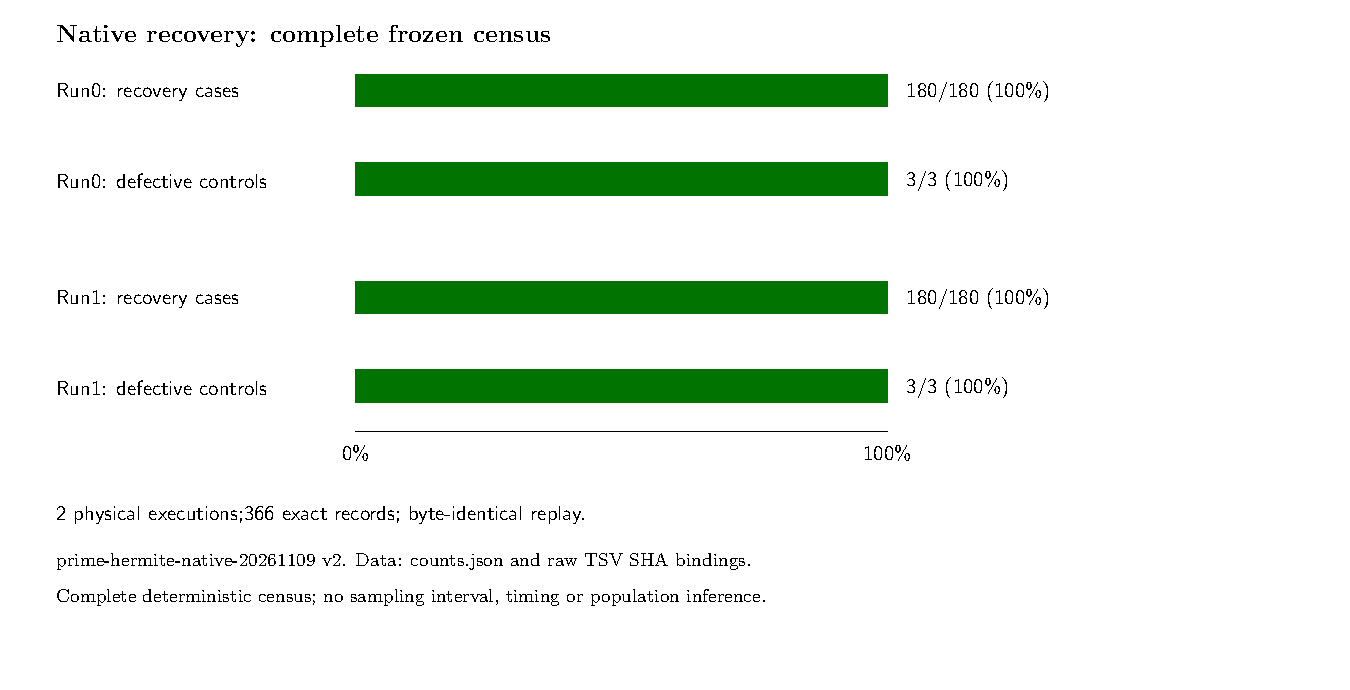
\includegraphics[width=\linewidth]{../native-20261109/plot.pdf}

\textbf{Workload.} Five triples$(a,u,M)$, three immutable sparse weight
fixtures, two injective placements, output precisions1/4/9 and canonical/offset
lifts give180 positive cases. The $a=4$ domain is held out relative to $a=3$
development. All actual active source nodes and original child precisions are
used. Exact source and binary hashes are frozen; C++20/GMP6.3.0, g++14.2.0.

\textbf{Controls.} Zero quotient misses delta target1; corrupting node1's
quotient constant by one yields nonintegrality; a scalar affine control
separates $D-N=1$ from $1-N=-1$ at $D=3,N=2$. The affine control tests that
identity, not an entire faulty contraction implementation. Full second
invocation is A/A; exact byte spread zero.
\newpage
{\Large Methods, provenance and limits}\par
\begin{center}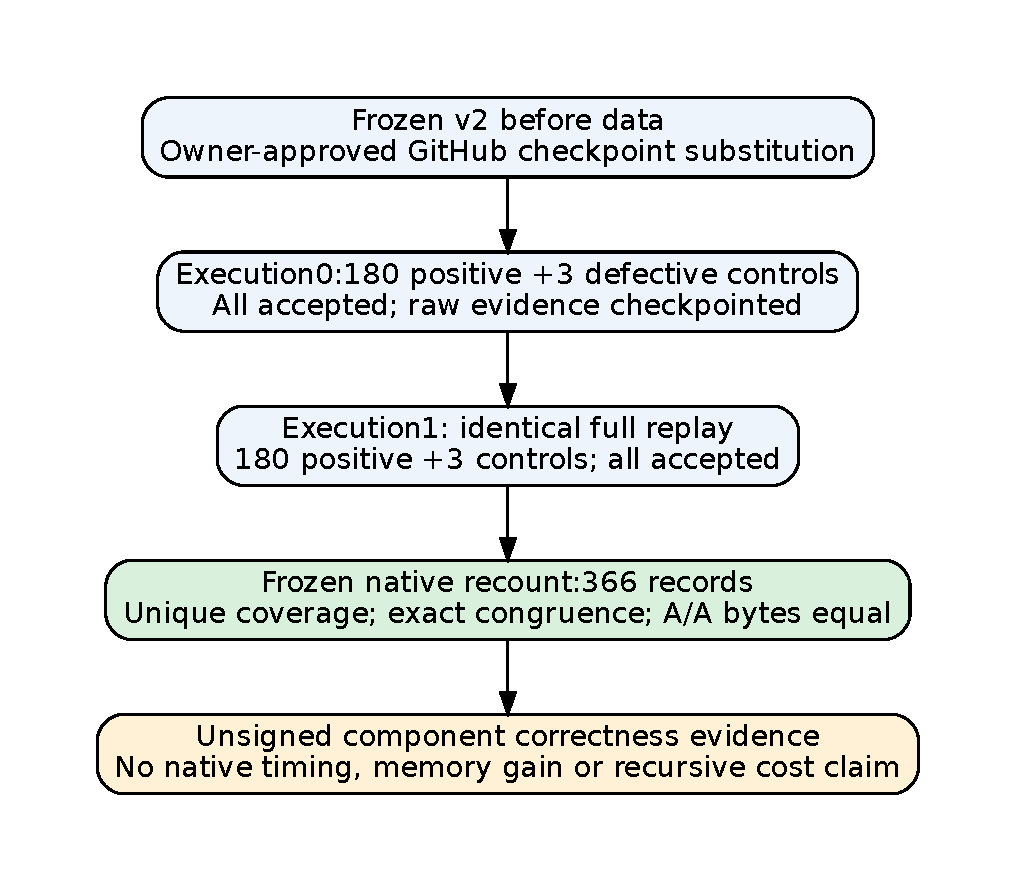
\includegraphics[width=0.9\linewidth,height=0.43\textheight,keepaspectratio]{flow.pdf}\end{center}

\textbf{Instrument.} Source \texttt{77aed44a5}; unchanged checker and analyzer.
The checker uses actual affine clearing, dense small-fixture polynomial charts,
finite modular inverse/convolution, integer lifts and a rational Hermite sum.
The analyzer uses numerator-minus-target-times-denominator divisibility,
separately from the checker's denominator inversion.

\textbf{Admission.} Owner approved GitHub checkpoints instead of unavailable
S3. Exact protocolv1 is retained; v2 changes only checkpoint transport before
data. Freeze20:07:22UTC; lifecycle markers run0 20:07:42--20:07:49,
run1 20:07:53--20:08:00. These are provenance, not timing measurements.
Local Linux x86-64/AMD EPYC9V74 model; each single-thread checker pinned to
CPU0,2GiB address-space cap,600s timeout,32MiB output cap; no retries.
Analyzer1CPU/2GiB/60s. Host co-tenants not isolated, L0, clocks invalid.

\textbf{Evidence.} Raw panels and receipts in \texttt{../../runs/}; native
recount \texttt{../../summary.json}; canonical two-row \texttt{../../export.json}.
Schema and native artifact bindings pass. Both raw TSV SHA256 values:
\nolinkurl{46a73583d9709c64acbcf02fbadb82734ed48b16cb5c33d85341ca74db512c09}.
Protocol hash:
\nolinkurl{7d5b77252d2930a0e8da185f08e0454809af934270dfa94c1a1a44bd50d57635}.

\textbf{Scope.} Finite native component correctness only. No timing, measured
memory-saving, full recursive runtime or curve solve result. Same-producer
recount/replay is not independent signed verification. Next: native refinement
of the distinct modular accumulator under a prospective amendment.
Sources are actual formal recovery and pinned manuscript D.9/D.10; KB unavailable.
\end{document}
